\ylDisplay{Elektriskeem} % Ülesande nimi
{Oleg Košik} % Autor
{piirkonnavoor} % Voor
{2013} % Aasta
{G 5} % Ülesande nr.
{3} % Raskustase
{
% Teema: Elektriahelad
\ifStatement
\begin{wrapfigure}[7]{r}{2.5cm}%
\vspace{-12pt}
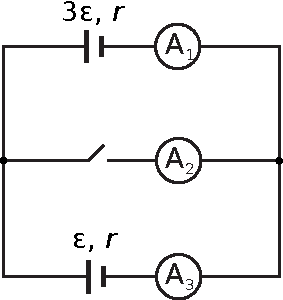
\includegraphics[width=\linewidth]{2013-v2g-05-skeem}%
\end{wrapfigure}
Joonisel toodud skeemil on ampermeetrid ideaalsed; patareide elektromotoorjõud
ja sisetakistused on märgitud nende juurde. Leidke ampermeetrite näidud, kui\\
\osa lüliti on suletud;\\
\osa lüliti on lahti.\\
\emph{Märkus}. praktikas tohib
sellist skeemi kasutada vaid siis, kui ollakse veendunud, et tekkivad voolud
jäävad ampermeetrite mõõtepiirkonda!
\fi


\ifHint
Mõlema kontuuri jaoks saab rakendada Ohmi seadust või Kirchhoffi seadusi.
\fi


\ifSolution
\osa Tekib kaks kontuuri, milles igaühes on üks vooluallikas ning kaks ampermeetrit. Voolud ampermeetritel 1 ja 3 leiame Ohmi seadusest: $I_1=\frac{3\varepsilon}{r}$, $I_3=\frac{\varepsilon}{r}$, voolu ampermeetril 2 aga Kirchhoffi I seadusest: 
\[
I_2=I_1+I_3=\frac{4\varepsilon}{r}.
\]

\osa Ilmselt $I_2=0$. Tekib üks kontuur, mis sisaldab kahte vooluallikat. Voolutugevuse kontuuris leiame Kirchhoffi II seadusest:
\[
I_1=I_3=\frac{3\varepsilon-\varepsilon}{r+r}=\frac{\varepsilon}{r}.
\]
\fi


\ifEngStatement
% Problem name: Circuit diagram
\begin{wrapfigure}[7]{r}{2.5cm}%
\vspace{-15pt}
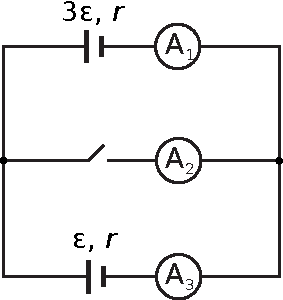
\includegraphics[width=\linewidth]{2013-v2g-05-skeem}%
\end{wrapfigure}
The ammeters in the circuit diagram given in the drawing are ideal; the electromotive forces and internal resistances of the batteries are marked in the drawing. Find the readings of the ammeters if\\
a) the switch is closed;\\
b) the switch is opened. (\emph{Note.}  In practice this circuit should be used only when it is certain that the appearing currents will stay in the regions measured by the ammeters!)
\fi


\ifEngHint
You can use the Ohm’s law or the Kirchhoff’s circuit laws for both of the contours.
\fi


\ifEngSolution
a) Two contours occur where each of them has one current source and two ammeters. We find the currents on the ammeters 1 and 3 through the Ohm’s law: $I_1=\frac{3\varepsilon}{r}$, $I_3=\frac{\varepsilon}{r}$, however, the current on the ammeter 2 we find through the Kirchhoff’s first law: $I_2=I_1+I_3=\frac{4\varepsilon}{r}$.\\
b) Probably $I_2=0$. One contour is formed and it contains two current sources. We find the current strength in the contour with the Kirchhoff’s second law:
\[
I_1=I_3=\frac{3\varepsilon-\varepsilon}{r+r}=\frac{\varepsilon}{r}.
\].
\fi
}